% -*- coding: utf-8 -*-
%-------------------------designed by zcf--------------
\documentclass[UTF8,a4paper,10pt]{ctexart}
\usepackage[left=3.17cm, right=3.17cm, top=2.74cm, bottom=2.74cm]{geometry}
\usepackage{amsmath}
\usepackage{graphicx,subfig}
\usepackage{float}
\usepackage{cite}
\usepackage{caption}
\usepackage{enumerate}
\usepackage{pythonhighlight}
\usepackage{booktabs} %表格
\usepackage{multirow}
\newcommand{\tabincell}[2]{\begin{tabular}{@{}#1@{}}#2\end{tabular}}  %表格强制换行
%-------------------------字体设置--------------
\usepackage{times} 
\newcommand{\yihao}{\fontsize{26pt}{36pt}\selectfont}           % 一号, 1.4 倍行距
\newcommand{\erhao}{\fontsize{22pt}{28pt}\selectfont}          % 二号, 1.25倍行距
\newcommand{\xiaoer}{\fontsize{18pt}{18pt}\selectfont}          % 小二, 单倍行距
\newcommand{\sanhao}{\fontsize{16pt}{24pt}\selectfont}  %三号字
\newcommand{\xiaosan}{\fontsize{15pt}{22pt}\selectfont}        % 小三, 1.5倍行距
\newcommand{\sihao}{\fontsize{14pt}{21pt}\selectfont}            % 四号, 1.5 倍行距
\newcommand{\banxiaosi}{\fontsize{13pt}{19.5pt}\selectfont}    % 半小四, 1.5倍行距
\newcommand{\xiaosi}{\fontsize{12pt}{18pt}\selectfont}            % 小四, 1.5倍行距
\newcommand{\dawuhao}{\fontsize{11pt}{11pt}\selectfont}       % 大五号, 单倍行距
\newcommand{\wuhao}{\fontsize{10.5pt}{15.75pt}\selectfont}    % 五号, 单倍行距
%-------------------------章节名----------------
\usepackage{ctexcap} 
\CTEXsetup[name={,、},number={ \chinese{section}}]{section}
\CTEXsetup[name={(,)},number={\chinese{subsection}}]{subsection}
\CTEXsetup[name={,.},number={\arabic{subsubsection}}]{subsubsection}
%-------------------------页眉页脚--------------
\usepackage{fancyhdr}
\pagestyle{fancy}
\lhead{\kaishu \leftmark}
% \chead{}
\rhead{\kaishu 机器学习实验报告}%加粗\bfseries 
\lfoot{}
\cfoot{\thepage}
\rfoot{}
\renewcommand{\headrulewidth}{0.1pt}  
\renewcommand{\footrulewidth}{0pt}%去掉横线
\newcommand{\HRule}{\rule{\linewidth}{0.5mm}}%标题横线
\newcommand{\HRulegrossa}{\rule{\linewidth}{1.2mm}}
%-----------------------伪代码------------------
\usepackage{algorithm}  
\usepackage{algorithmicx}  
\usepackage{algpseudocode}  
\floatname{algorithm}{Algorithm}  
\renewcommand{\algorithmicrequire}{\textbf{Input:}}  
\renewcommand{\algorithmicensure}{\textbf{Output:}} 
\usepackage{lipsum}  
\makeatletter
\newenvironment{breakablealgorithm}
  {% \begin{breakablealgorithm}
  \begin{center}
     \refstepcounter{algorithm}% New algorithm
     \hrule height.8pt depth0pt \kern2pt% \@fs@pre for \@fs@ruled
     \renewcommand{\caption}[2][\relax]{% Make a new \caption
      {\raggedright\textbf{\ALG@name~\thealgorithm} ##2\par}%
      \ifx\relax##1\relax % #1 is \relax
         \addcontentsline{loa}{algorithm}{\protect\numberline{\thealgorithm}##2}%
      \else % #1 is not \relax
         \addcontentsline{loa}{algorithm}{\protect\numberline{\thealgorithm}##1}%
      \fi
      \kern2pt\hrule\kern2pt
     }
  }{% \end{breakablealgorithm}
     \kern2pt\hrule\relax% \@fs@post for \@fs@ruled
  \end{center}
  }
\makeatother
%------------------------代码-------------------
\usepackage{xcolor} 
\usepackage{listings} 
\lstset{ 
breaklines,%自动换行
basicstyle=\small,
escapeinside=``,
keywordstyle=\color{ blue!70} \bfseries,
commentstyle=\color{red!50!green!50!blue!50},% 
stringstyle=\ttfamily,% 
extendedchars=false,% 
linewidth=\textwidth,% 
numbers=left,% 
numberstyle=\tiny \color{blue!50},% 
frame=trbl% 
rulesepcolor= \color{ red!20!green!20!blue!20} 
}
%------------超链接----------
\usepackage[colorlinks,linkcolor=black,anchorcolor=blue]{hyperref}
%------------------------TODO-------------------
\usepackage{enumitem,amssymb}
\newlist{todolist}{itemize}{2}
\setlist[todolist]{label=$\square$}
% for check symbol 
\usepackage{pifont}
\newcommand{\cmark}{\ding{51}}%
\newcommand{\xmark}{\ding{55}}%
\newcommand{\done}{\rlap{$\square$}{\raisebox{2pt}{\large\hspace{1pt}\cmark}}\hspace{-2.5pt}}
\newcommand{\wontfix}{\rlap{$\square$}{\large\hspace{1pt}\xmark}}
%------------------------水印-------------------
\usepackage{tikz}
\usepackage{xcolor}
\usepackage{eso-pic}

\newcommand{\watermark}[3]{\AddToShipoutPictureBG{
\parbox[b][\paperheight]{\paperwidth}{
\vfill%
\centering%
\tikz[remember picture, overlay]%
  \node [rotate = #1, scale = #2] at (current page.center)%
    {\textcolor{gray!80!cyan!30!magenta!30}{#3}};
\vfill}}}



%———————————————————————————————————————————正文———————————————————————————————————————————————
%----------------------------------------------
\begin{document}
\begin{titlepage}
    \begin{center}
    
\includegraphics[width=0.8\textwidth]{NKU.png}\\[1cm]    
    \textsc{\Huge \kaishu{\textbf{南\ \ \ \ \ \ 开\ \ \ \ \ \ 大\ \ \ \ \ \ 学}} }\\[0.9cm]
    \textsc{\huge \kaishu{\textbf{计\ \ 算\ \ 机\ \ 学\ \ 院}}}\\[0.5cm]
    \textsc{\Large \textbf{机器学习实验报告}}\\[0.8cm]
    \HRule \\[0.9cm]
    { \LARGE \bfseries 实验二\ 回归模型}\\[0.4cm]
    \HRule \\[2.0cm]
    \centering
    \textsc{\LARGE \kaishu{姓名\ :\ 王泳鑫}}\\[0.5cm]
    \textsc{\LARGE \kaishu{学号\ :\ 1911479}}\\[0.5cm]
    \textsc{\LARGE \kaishu{年级\ :\ 2019级}}\\[0.5cm]
    \textsc{\LARGE \kaishu{专业\ :\ 计算机科学与技术}}\\[0.5cm]
    \textsc{\LARGE \kaishu{指导教师\ :\ 卫金茂}}\\[0.5cm]
    \vfill
    {\Large \today}
    \end{center}
\end{titlepage}
%-------------摘------要--------------
\newpage
\thispagestyle{empty}
\renewcommand{\abstractname}{\kaishu \sihao \textbf{摘要}}
    \begin{abstract}

        \noindent  %顶格
        \textbf{\\\ 关键字:线性回归,多元线性回归 ,Machine Learning , Deep Learning}\textbf{} \\\ \\\
    \end{abstract}
%----------------------------------------------------------------
\tableofcontents
%----------------------------------------------------------------
\newpage
\watermark{60}{10}{NKU}
\setcounter{page}{1}
%——————————————————————————————————————
\section{实验描述}
\subsection{实验内容}
利用课上所学实现线性回归模型,来完成以下实验要求。
\subsection{实验要求}
基本要求:

1.根据数据集dataset\_regression.csv,求最小二乘解,用得到的回归方程生成五个测试样本,画出回归曲线,给出训练误差。

2.将数据集winequality\_white.csv按照4:1划分为训练集和测试集,
构造线性回归模型,采用批量梯度下降或者随机梯度下降均可;输出训练集和测试集的均方误差(MSE),
画出MSE收敛曲线。

中级要求:

尝试不同的学习率并进行MSE曲线展示、分析选择最佳的学习率。
%——————————————————————————————————————
\section{代码实现}
\subsection{实验要求1与结果展示}
根据数据集dataset\_regression.csv,在利用最小二乘法时,我们得到x和y,但是在求解逆矩阵时,发现矩阵不存在逆矩阵,如下图\ref{fig:1}所示
\begin{figure}[H]
    \centering
    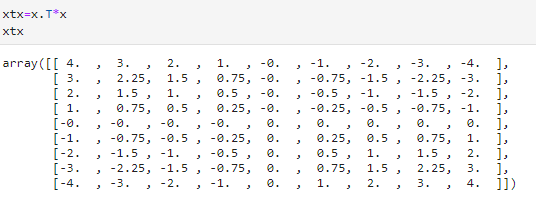
\includegraphics[scale=1]{1.png}
    \caption{无法求逆的矩阵}
    \label{fig:1}
\end{figure}

这个矩阵无法求逆,所以我们只能放弃最小二乘法,采用批量梯度下降,求解回归曲线。
也可以通过scipy库里的leastsq最小二乘法,代码如下:

首先是数据集的导入,并且把数据集中的第二列和第三列划分为x和y,代码如下:
\begin{python}
   dataset = np.loadtxt('D:\\Data\\dataset_regression.csv',float,delimiter=',',skiprows=1,usecols=(1,2))
   x=dataset[:,0]
   y=dataset[:,1]

\end{python}

接下来就是,规范我们要拟合的曲线的形式了,代码如下:

\begin{python}
   ##需要拟合的函数func :指定函数的形状

def func(p, x):
    k, b = p

    return k * x + b


##偏差函数:x,y都是列表:这里的x,y更上面的Xi,Yi中是一一对应的

def error(p, x, y):
    return func(p, x) - y

\end{python}

leastsq函数返回值第一个表示拟合结果,第二个表示最后的误差:

\begin{python}
   Para = leastsq(error, p0, args=(Xi, Yi))
\end{python}

经过拟合后,我们得到的最终结果如下图\ref{fig:1}所示:

\begin{figure}[H]
    \centering
    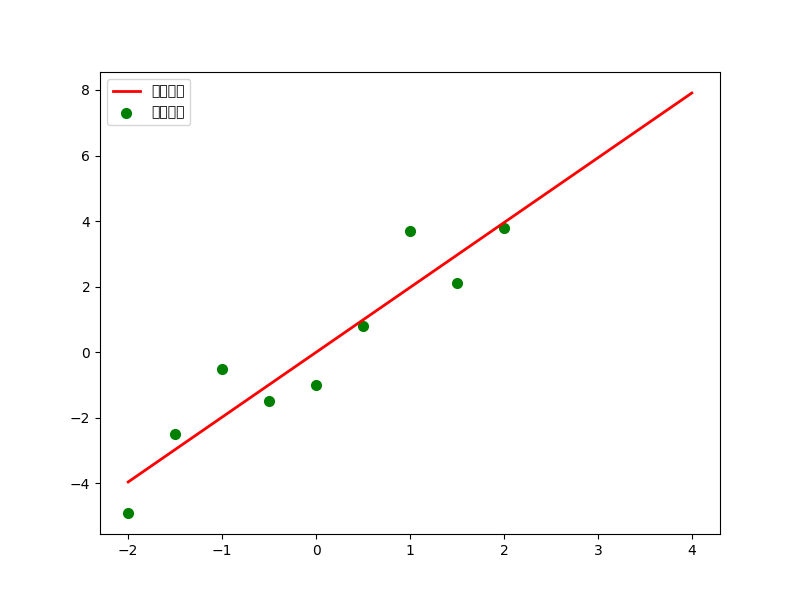
\includegraphics[scale=0.5]{2.png}
    \caption{拟合结果}
    \label{fig:1}
\end{figure}

拟合函数的数值和误差如下图\ref{fig:1}所示:

\begin{figure}[H]
    \centering
    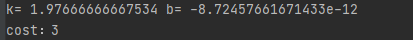
\includegraphics[scale=1]{3.png}
    \caption{拟合结果}
    \label{fig:1}
\end{figure}



\subsection{实验要求2}
本实验将数据集按照4:1划分为训练集和测试集,在这里,我通过留一法来划分,代码如下:

\begin{python}
   def loo_split(data, label, idx):
    train_data = []
    test_data = []
    train_label = []
    test_label = []
    for i in range(0, idx):
        train_data.append(data[i])
        train_label.append(label[i])
    test_data.append(data[idx])
    test_label.append(label[idx])
    for i in range(idx+1, data.shape[0]):
        train_data.append(data[i])
        train_label.append(label[i])
    return np.array(train_data), np.array(train_label), \
           np.array(test_data), np.array(test_label)

\end{python}

在实验要求2中,我利用随机梯度下降来完成线性回归,代码如下:

\begin{python}
   def linear_regression(data, label, lr, epochs, reg=None, alpha=None, random=False):
    data = data_normalization(data)
    preds = []
    for i in range(data.shape[0]):  # 每一条数据都要用留一法进行预测
        train_data, train_label, test_data, test_label = loo_split(data, label, i)
        errors, weight = gradient_descent(train_data, train_label, lr, epochs, reg, alpha, random)
        test_x = np.hstack((np.array([1]).reshape((1, 1)), test_data))
        pred_y = np.dot(test_x, weight)
        preds.append(pred_y)
        if i % 100 == 0:
            print(i, 'loo')
    preds = np.array(preds).reshape(label.shape)
    rmse = np.sqrt(((preds - label) ** 2).mean())  # 计算所有预测值的RMSE
    return preds, rmse, errors
\end{python}

其中我们要先把数据标准化,代码如下:


\begin{python}
   def data_normalization(data):
    data_normed = data
    for i in range(data.shape[1]):
        cur_col = data[:, i]
        mean = np.mean(cur_col)
        std = np.std(cur_col)
        for j in range(cur_col.shape[0]):
            data_normed[j, i] = (data[j, i] - mean) / std
    return data_normed
\end{python}

然后对于每一条数据都要进行一次留一法进行预测,然后对训练集进行梯度下降的计算,同时返回误差和权重,代码如下:

\begin{python}
   def gradient_descent(data, label, lr, epochs, reg=None, alpha=None, random=False):
    weight = np.zeros((12))  # 在11个特征列基础上加一个常数项
    x = np.hstack((np.ones((data.shape[0], 1)), data))  # 给数据加上全1的一列
    y = label
    errors = []
    if reg is None:
        for epoch in range(epochs):
            error, grad = gradient(weight, x, y, random)
            weight = weight - lr * grad
            errors.append(error)
    elif reg == 'L1':
        for epoch in range(epochs):
            error, grad = gradient_L1(weight, x, y, alpha, random)
            weight = weight - lr * grad
            errors.append(error)
    else:
        for epoch in range(epochs):
            error, grad = gradient_L2(weight, x, y, alpha, random)
            weight = weight - lr * grad
            errors.append(error)
    return errors, weight
\end{python}

对于梯度下降的计算,我采用了三个不同loss函数计算来优化梯度下降,代码如下:

\begin{python}
   def gradient(weight, x, y, random=False):
    if random is False:
        error = np.dot(x, weight) - y
        return abs(error.mean()), (1/x.shape[0]) * np.dot(np.transpose(x), error)  # 注意各个矩阵维度的匹配
    else:
        rand = np.random.randint(0, x.shape[0] - 1)  # 用numpy中的方法生成随机数
        x_rand = x[rand, :]
        y_rand = y[rand]
        error = np.dot(x_rand, weight) - y_rand
        return abs(error.mean()), (1/x.shape[0]) * np.dot(x_rand, error)


def gradient_L1(weight, x, y, alpha, random=False):
    if random is False:
        error = np.dot(x, weight) - y
        return abs(error.mean()), (1/x.shape[0]) * (np.dot(np.transpose(x), error)
                                                    + alpha * np.sign(weight))  # 正则项求导后为sign(x)
    else:
        rand = np.random.randint(0, x.shape[0] - 1)
        x_rand = x[rand, :]
        y_rand = y[rand]
        error = np.dot(x_rand, weight) - y_rand
        return abs(error.mean()), (1/x.shape[0]) * (np.dot(x_rand, error) + alpha * np.sign(weight))


def gradient_L2(weight, x, y, alpha, random=False):
    if random is False:
        error = np.dot(x, weight) - y
        # 正则项求导后为weight值的一次形式
        return abs(error.mean()), (1/x.shape[0]) * (np.dot(np.transpose(x), error) + alpha * weight)
    else:
        rand = np.random.randint(0, x.shape[0] - 1)
        x_rand = x[rand, :]
        y_rand = y[rand]
        error = np.dot(x_rand, weight) - y_rand
        return abs(error.mean()), (1/x.shape[0]) * (np.dot(x_rand, error) + alpha * weight)
\end{python}

实验结果如下图\ref{fig:1}所示:

\begin{figure}[H]
    \centering
    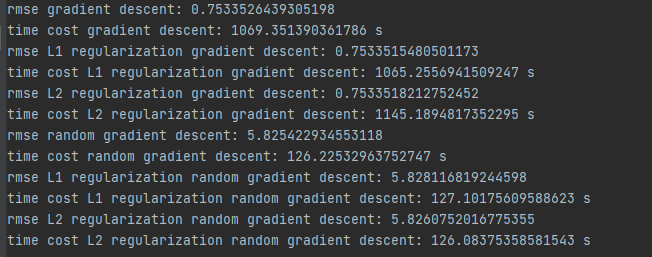
\includegraphics[scale=0.7]{5.png}
    \caption{实验结果}
    \label{fig:1}
\end{figure}

误差和迭代次数的关系如下图\ref{fig:1}所示:

\begin{figure}[H]
    \centering
    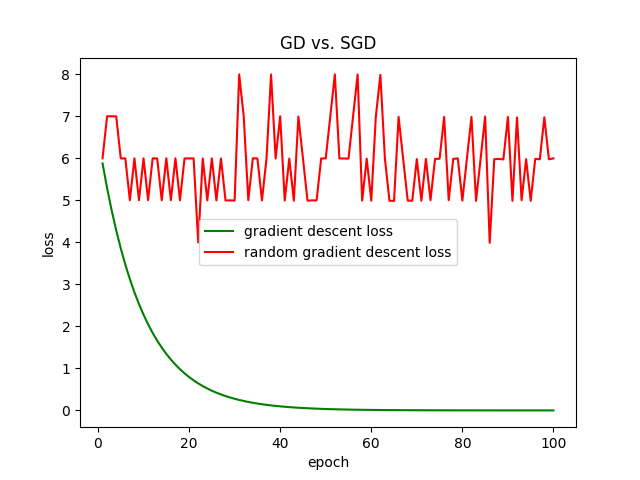
\includegraphics[scale=0.5]{4.png}
    \caption{关系}
    \label{fig:1}
\end{figure}



%——————————————————————————————————————



%----------------------------------------------------------------

%----------------------------------------------------------------
\bibliographystyle{plain}
\end{document}
